
% Default to the notebook output style

    


% Inherit from the specified cell style.




    
\documentclass[11pt]{article}

    
    
    \usepackage[T1]{fontenc}
    % Nicer default font (+ math font) than Computer Modern for most use cases
    \usepackage{mathpazo}

    % Basic figure setup, for now with no caption control since it's done
    % automatically by Pandoc (which extracts ![](path) syntax from Markdown).
    \usepackage{graphicx}
    % We will generate all images so they have a width \maxwidth. This means
    % that they will get their normal width if they fit onto the page, but
    % are scaled down if they would overflow the margins.
    \makeatletter
    \def\maxwidth{\ifdim\Gin@nat@width>\linewidth\linewidth
    \else\Gin@nat@width\fi}
    \makeatother
    \let\Oldincludegraphics\includegraphics
    % Set max figure width to be 80% of text width, for now hardcoded.
    \renewcommand{\includegraphics}[1]{\Oldincludegraphics[width=.8\maxwidth]{#1}}
    % Ensure that by default, figures have no caption (until we provide a
    % proper Figure object with a Caption API and a way to capture that
    % in the conversion process - todo).
    \usepackage{caption}
    \DeclareCaptionLabelFormat{nolabel}{}
    \captionsetup{labelformat=nolabel}

    \usepackage{adjustbox} % Used to constrain images to a maximum size 
    \usepackage{xcolor} % Allow colors to be defined
    \usepackage{enumerate} % Needed for markdown enumerations to work
    \usepackage{geometry} % Used to adjust the document margins
    \usepackage{amsmath} % Equations
    \usepackage{amssymb} % Equations
    \usepackage{textcomp} % defines textquotesingle
    % Hack from http://tex.stackexchange.com/a/47451/13684:
    \AtBeginDocument{%
        \def\PYZsq{\textquotesingle}% Upright quotes in Pygmentized code
    }
    \usepackage{upquote} % Upright quotes for verbatim code
    \usepackage{eurosym} % defines \euro
    \usepackage[mathletters]{ucs} % Extended unicode (utf-8) support
    \usepackage[utf8x]{inputenc} % Allow utf-8 characters in the tex document
    \usepackage{fancyvrb} % verbatim replacement that allows latex
    \usepackage{grffile} % extends the file name processing of package graphics 
                         % to support a larger range 
    % The hyperref package gives us a pdf with properly built
    % internal navigation ('pdf bookmarks' for the table of contents,
    % internal cross-reference links, web links for URLs, etc.)
    \usepackage{hyperref}
    \usepackage{longtable} % longtable support required by pandoc >1.10
    \usepackage{booktabs}  % table support for pandoc > 1.12.2
    \usepackage[inline]{enumitem} % IRkernel/repr support (it uses the enumerate* environment)
    \usepackage[normalem]{ulem} % ulem is needed to support strikethroughs (\sout)
                                % normalem makes italics be italics, not underlines
    

    
    
    % Colors for the hyperref package
    \definecolor{urlcolor}{rgb}{0,.145,.698}
    \definecolor{linkcolor}{rgb}{.71,0.21,0.01}
    \definecolor{citecolor}{rgb}{.12,.54,.11}

    % ANSI colors
    \definecolor{ansi-black}{HTML}{3E424D}
    \definecolor{ansi-black-intense}{HTML}{282C36}
    \definecolor{ansi-red}{HTML}{E75C58}
    \definecolor{ansi-red-intense}{HTML}{B22B31}
    \definecolor{ansi-green}{HTML}{00A250}
    \definecolor{ansi-green-intense}{HTML}{007427}
    \definecolor{ansi-yellow}{HTML}{DDB62B}
    \definecolor{ansi-yellow-intense}{HTML}{B27D12}
    \definecolor{ansi-blue}{HTML}{208FFB}
    \definecolor{ansi-blue-intense}{HTML}{0065CA}
    \definecolor{ansi-magenta}{HTML}{D160C4}
    \definecolor{ansi-magenta-intense}{HTML}{A03196}
    \definecolor{ansi-cyan}{HTML}{60C6C8}
    \definecolor{ansi-cyan-intense}{HTML}{258F8F}
    \definecolor{ansi-white}{HTML}{C5C1B4}
    \definecolor{ansi-white-intense}{HTML}{A1A6B2}

    % commands and environments needed by pandoc snippets
    % extracted from the output of `pandoc -s`
    \providecommand{\tightlist}{%
      \setlength{\itemsep}{0pt}\setlength{\parskip}{0pt}}
    \DefineVerbatimEnvironment{Highlighting}{Verbatim}{commandchars=\\\{\}}
    % Add ',fontsize=\small' for more characters per line
    \newenvironment{Shaded}{}{}
    \newcommand{\KeywordTok}[1]{\textcolor[rgb]{0.00,0.44,0.13}{\textbf{{#1}}}}
    \newcommand{\DataTypeTok}[1]{\textcolor[rgb]{0.56,0.13,0.00}{{#1}}}
    \newcommand{\DecValTok}[1]{\textcolor[rgb]{0.25,0.63,0.44}{{#1}}}
    \newcommand{\BaseNTok}[1]{\textcolor[rgb]{0.25,0.63,0.44}{{#1}}}
    \newcommand{\FloatTok}[1]{\textcolor[rgb]{0.25,0.63,0.44}{{#1}}}
    \newcommand{\CharTok}[1]{\textcolor[rgb]{0.25,0.44,0.63}{{#1}}}
    \newcommand{\StringTok}[1]{\textcolor[rgb]{0.25,0.44,0.63}{{#1}}}
    \newcommand{\CommentTok}[1]{\textcolor[rgb]{0.38,0.63,0.69}{\textit{{#1}}}}
    \newcommand{\OtherTok}[1]{\textcolor[rgb]{0.00,0.44,0.13}{{#1}}}
    \newcommand{\AlertTok}[1]{\textcolor[rgb]{1.00,0.00,0.00}{\textbf{{#1}}}}
    \newcommand{\FunctionTok}[1]{\textcolor[rgb]{0.02,0.16,0.49}{{#1}}}
    \newcommand{\RegionMarkerTok}[1]{{#1}}
    \newcommand{\ErrorTok}[1]{\textcolor[rgb]{1.00,0.00,0.00}{\textbf{{#1}}}}
    \newcommand{\NormalTok}[1]{{#1}}
    
    % Additional commands for more recent versions of Pandoc
    \newcommand{\ConstantTok}[1]{\textcolor[rgb]{0.53,0.00,0.00}{{#1}}}
    \newcommand{\SpecialCharTok}[1]{\textcolor[rgb]{0.25,0.44,0.63}{{#1}}}
    \newcommand{\VerbatimStringTok}[1]{\textcolor[rgb]{0.25,0.44,0.63}{{#1}}}
    \newcommand{\SpecialStringTok}[1]{\textcolor[rgb]{0.73,0.40,0.53}{{#1}}}
    \newcommand{\ImportTok}[1]{{#1}}
    \newcommand{\DocumentationTok}[1]{\textcolor[rgb]{0.73,0.13,0.13}{\textit{{#1}}}}
    \newcommand{\AnnotationTok}[1]{\textcolor[rgb]{0.38,0.63,0.69}{\textbf{\textit{{#1}}}}}
    \newcommand{\CommentVarTok}[1]{\textcolor[rgb]{0.38,0.63,0.69}{\textbf{\textit{{#1}}}}}
    \newcommand{\VariableTok}[1]{\textcolor[rgb]{0.10,0.09,0.49}{{#1}}}
    \newcommand{\ControlFlowTok}[1]{\textcolor[rgb]{0.00,0.44,0.13}{\textbf{{#1}}}}
    \newcommand{\OperatorTok}[1]{\textcolor[rgb]{0.40,0.40,0.40}{{#1}}}
    \newcommand{\BuiltInTok}[1]{{#1}}
    \newcommand{\ExtensionTok}[1]{{#1}}
    \newcommand{\PreprocessorTok}[1]{\textcolor[rgb]{0.74,0.48,0.00}{{#1}}}
    \newcommand{\AttributeTok}[1]{\textcolor[rgb]{0.49,0.56,0.16}{{#1}}}
    \newcommand{\InformationTok}[1]{\textcolor[rgb]{0.38,0.63,0.69}{\textbf{\textit{{#1}}}}}
    \newcommand{\WarningTok}[1]{\textcolor[rgb]{0.38,0.63,0.69}{\textbf{\textit{{#1}}}}}
    
    
    % Define a nice break command that doesn't care if a line doesn't already
    % exist.
    \def\br{\hspace*{\fill} \\* }
    % Math Jax compatability definitions
    \def\gt{>}
    \def\lt{<}
    % Document parameters
    \title{Exercise 2  Gradient Method}
    
    
    

    % Pygments definitions
    
\makeatletter
\def\PY@reset{\let\PY@it=\relax \let\PY@bf=\relax%
    \let\PY@ul=\relax \let\PY@tc=\relax%
    \let\PY@bc=\relax \let\PY@ff=\relax}
\def\PY@tok#1{\csname PY@tok@#1\endcsname}
\def\PY@toks#1+{\ifx\relax#1\empty\else%
    \PY@tok{#1}\expandafter\PY@toks\fi}
\def\PY@do#1{\PY@bc{\PY@tc{\PY@ul{%
    \PY@it{\PY@bf{\PY@ff{#1}}}}}}}
\def\PY#1#2{\PY@reset\PY@toks#1+\relax+\PY@do{#2}}

\expandafter\def\csname PY@tok@gd\endcsname{\def\PY@tc##1{\textcolor[rgb]{0.63,0.00,0.00}{##1}}}
\expandafter\def\csname PY@tok@gu\endcsname{\let\PY@bf=\textbf\def\PY@tc##1{\textcolor[rgb]{0.50,0.00,0.50}{##1}}}
\expandafter\def\csname PY@tok@gt\endcsname{\def\PY@tc##1{\textcolor[rgb]{0.00,0.27,0.87}{##1}}}
\expandafter\def\csname PY@tok@gs\endcsname{\let\PY@bf=\textbf}
\expandafter\def\csname PY@tok@gr\endcsname{\def\PY@tc##1{\textcolor[rgb]{1.00,0.00,0.00}{##1}}}
\expandafter\def\csname PY@tok@cm\endcsname{\let\PY@it=\textit\def\PY@tc##1{\textcolor[rgb]{0.25,0.50,0.50}{##1}}}
\expandafter\def\csname PY@tok@vg\endcsname{\def\PY@tc##1{\textcolor[rgb]{0.10,0.09,0.49}{##1}}}
\expandafter\def\csname PY@tok@vi\endcsname{\def\PY@tc##1{\textcolor[rgb]{0.10,0.09,0.49}{##1}}}
\expandafter\def\csname PY@tok@vm\endcsname{\def\PY@tc##1{\textcolor[rgb]{0.10,0.09,0.49}{##1}}}
\expandafter\def\csname PY@tok@mh\endcsname{\def\PY@tc##1{\textcolor[rgb]{0.40,0.40,0.40}{##1}}}
\expandafter\def\csname PY@tok@cs\endcsname{\let\PY@it=\textit\def\PY@tc##1{\textcolor[rgb]{0.25,0.50,0.50}{##1}}}
\expandafter\def\csname PY@tok@ge\endcsname{\let\PY@it=\textit}
\expandafter\def\csname PY@tok@vc\endcsname{\def\PY@tc##1{\textcolor[rgb]{0.10,0.09,0.49}{##1}}}
\expandafter\def\csname PY@tok@il\endcsname{\def\PY@tc##1{\textcolor[rgb]{0.40,0.40,0.40}{##1}}}
\expandafter\def\csname PY@tok@go\endcsname{\def\PY@tc##1{\textcolor[rgb]{0.53,0.53,0.53}{##1}}}
\expandafter\def\csname PY@tok@cp\endcsname{\def\PY@tc##1{\textcolor[rgb]{0.74,0.48,0.00}{##1}}}
\expandafter\def\csname PY@tok@gi\endcsname{\def\PY@tc##1{\textcolor[rgb]{0.00,0.63,0.00}{##1}}}
\expandafter\def\csname PY@tok@gh\endcsname{\let\PY@bf=\textbf\def\PY@tc##1{\textcolor[rgb]{0.00,0.00,0.50}{##1}}}
\expandafter\def\csname PY@tok@ni\endcsname{\let\PY@bf=\textbf\def\PY@tc##1{\textcolor[rgb]{0.60,0.60,0.60}{##1}}}
\expandafter\def\csname PY@tok@nl\endcsname{\def\PY@tc##1{\textcolor[rgb]{0.63,0.63,0.00}{##1}}}
\expandafter\def\csname PY@tok@nn\endcsname{\let\PY@bf=\textbf\def\PY@tc##1{\textcolor[rgb]{0.00,0.00,1.00}{##1}}}
\expandafter\def\csname PY@tok@no\endcsname{\def\PY@tc##1{\textcolor[rgb]{0.53,0.00,0.00}{##1}}}
\expandafter\def\csname PY@tok@na\endcsname{\def\PY@tc##1{\textcolor[rgb]{0.49,0.56,0.16}{##1}}}
\expandafter\def\csname PY@tok@nb\endcsname{\def\PY@tc##1{\textcolor[rgb]{0.00,0.50,0.00}{##1}}}
\expandafter\def\csname PY@tok@nc\endcsname{\let\PY@bf=\textbf\def\PY@tc##1{\textcolor[rgb]{0.00,0.00,1.00}{##1}}}
\expandafter\def\csname PY@tok@nd\endcsname{\def\PY@tc##1{\textcolor[rgb]{0.67,0.13,1.00}{##1}}}
\expandafter\def\csname PY@tok@ne\endcsname{\let\PY@bf=\textbf\def\PY@tc##1{\textcolor[rgb]{0.82,0.25,0.23}{##1}}}
\expandafter\def\csname PY@tok@nf\endcsname{\def\PY@tc##1{\textcolor[rgb]{0.00,0.00,1.00}{##1}}}
\expandafter\def\csname PY@tok@si\endcsname{\let\PY@bf=\textbf\def\PY@tc##1{\textcolor[rgb]{0.73,0.40,0.53}{##1}}}
\expandafter\def\csname PY@tok@s2\endcsname{\def\PY@tc##1{\textcolor[rgb]{0.73,0.13,0.13}{##1}}}
\expandafter\def\csname PY@tok@nt\endcsname{\let\PY@bf=\textbf\def\PY@tc##1{\textcolor[rgb]{0.00,0.50,0.00}{##1}}}
\expandafter\def\csname PY@tok@nv\endcsname{\def\PY@tc##1{\textcolor[rgb]{0.10,0.09,0.49}{##1}}}
\expandafter\def\csname PY@tok@s1\endcsname{\def\PY@tc##1{\textcolor[rgb]{0.73,0.13,0.13}{##1}}}
\expandafter\def\csname PY@tok@dl\endcsname{\def\PY@tc##1{\textcolor[rgb]{0.73,0.13,0.13}{##1}}}
\expandafter\def\csname PY@tok@ch\endcsname{\let\PY@it=\textit\def\PY@tc##1{\textcolor[rgb]{0.25,0.50,0.50}{##1}}}
\expandafter\def\csname PY@tok@m\endcsname{\def\PY@tc##1{\textcolor[rgb]{0.40,0.40,0.40}{##1}}}
\expandafter\def\csname PY@tok@gp\endcsname{\let\PY@bf=\textbf\def\PY@tc##1{\textcolor[rgb]{0.00,0.00,0.50}{##1}}}
\expandafter\def\csname PY@tok@sh\endcsname{\def\PY@tc##1{\textcolor[rgb]{0.73,0.13,0.13}{##1}}}
\expandafter\def\csname PY@tok@ow\endcsname{\let\PY@bf=\textbf\def\PY@tc##1{\textcolor[rgb]{0.67,0.13,1.00}{##1}}}
\expandafter\def\csname PY@tok@sx\endcsname{\def\PY@tc##1{\textcolor[rgb]{0.00,0.50,0.00}{##1}}}
\expandafter\def\csname PY@tok@bp\endcsname{\def\PY@tc##1{\textcolor[rgb]{0.00,0.50,0.00}{##1}}}
\expandafter\def\csname PY@tok@c1\endcsname{\let\PY@it=\textit\def\PY@tc##1{\textcolor[rgb]{0.25,0.50,0.50}{##1}}}
\expandafter\def\csname PY@tok@fm\endcsname{\def\PY@tc##1{\textcolor[rgb]{0.00,0.00,1.00}{##1}}}
\expandafter\def\csname PY@tok@o\endcsname{\def\PY@tc##1{\textcolor[rgb]{0.40,0.40,0.40}{##1}}}
\expandafter\def\csname PY@tok@kc\endcsname{\let\PY@bf=\textbf\def\PY@tc##1{\textcolor[rgb]{0.00,0.50,0.00}{##1}}}
\expandafter\def\csname PY@tok@c\endcsname{\let\PY@it=\textit\def\PY@tc##1{\textcolor[rgb]{0.25,0.50,0.50}{##1}}}
\expandafter\def\csname PY@tok@mf\endcsname{\def\PY@tc##1{\textcolor[rgb]{0.40,0.40,0.40}{##1}}}
\expandafter\def\csname PY@tok@err\endcsname{\def\PY@bc##1{\setlength{\fboxsep}{0pt}\fcolorbox[rgb]{1.00,0.00,0.00}{1,1,1}{\strut ##1}}}
\expandafter\def\csname PY@tok@mb\endcsname{\def\PY@tc##1{\textcolor[rgb]{0.40,0.40,0.40}{##1}}}
\expandafter\def\csname PY@tok@ss\endcsname{\def\PY@tc##1{\textcolor[rgb]{0.10,0.09,0.49}{##1}}}
\expandafter\def\csname PY@tok@sr\endcsname{\def\PY@tc##1{\textcolor[rgb]{0.73,0.40,0.53}{##1}}}
\expandafter\def\csname PY@tok@mo\endcsname{\def\PY@tc##1{\textcolor[rgb]{0.40,0.40,0.40}{##1}}}
\expandafter\def\csname PY@tok@kd\endcsname{\let\PY@bf=\textbf\def\PY@tc##1{\textcolor[rgb]{0.00,0.50,0.00}{##1}}}
\expandafter\def\csname PY@tok@mi\endcsname{\def\PY@tc##1{\textcolor[rgb]{0.40,0.40,0.40}{##1}}}
\expandafter\def\csname PY@tok@kn\endcsname{\let\PY@bf=\textbf\def\PY@tc##1{\textcolor[rgb]{0.00,0.50,0.00}{##1}}}
\expandafter\def\csname PY@tok@cpf\endcsname{\let\PY@it=\textit\def\PY@tc##1{\textcolor[rgb]{0.25,0.50,0.50}{##1}}}
\expandafter\def\csname PY@tok@kr\endcsname{\let\PY@bf=\textbf\def\PY@tc##1{\textcolor[rgb]{0.00,0.50,0.00}{##1}}}
\expandafter\def\csname PY@tok@s\endcsname{\def\PY@tc##1{\textcolor[rgb]{0.73,0.13,0.13}{##1}}}
\expandafter\def\csname PY@tok@kp\endcsname{\def\PY@tc##1{\textcolor[rgb]{0.00,0.50,0.00}{##1}}}
\expandafter\def\csname PY@tok@w\endcsname{\def\PY@tc##1{\textcolor[rgb]{0.73,0.73,0.73}{##1}}}
\expandafter\def\csname PY@tok@kt\endcsname{\def\PY@tc##1{\textcolor[rgb]{0.69,0.00,0.25}{##1}}}
\expandafter\def\csname PY@tok@sc\endcsname{\def\PY@tc##1{\textcolor[rgb]{0.73,0.13,0.13}{##1}}}
\expandafter\def\csname PY@tok@sb\endcsname{\def\PY@tc##1{\textcolor[rgb]{0.73,0.13,0.13}{##1}}}
\expandafter\def\csname PY@tok@sa\endcsname{\def\PY@tc##1{\textcolor[rgb]{0.73,0.13,0.13}{##1}}}
\expandafter\def\csname PY@tok@k\endcsname{\let\PY@bf=\textbf\def\PY@tc##1{\textcolor[rgb]{0.00,0.50,0.00}{##1}}}
\expandafter\def\csname PY@tok@se\endcsname{\let\PY@bf=\textbf\def\PY@tc##1{\textcolor[rgb]{0.73,0.40,0.13}{##1}}}
\expandafter\def\csname PY@tok@sd\endcsname{\let\PY@it=\textit\def\PY@tc##1{\textcolor[rgb]{0.73,0.13,0.13}{##1}}}

\def\PYZbs{\char`\\}
\def\PYZus{\char`\_}
\def\PYZob{\char`\{}
\def\PYZcb{\char`\}}
\def\PYZca{\char`\^}
\def\PYZam{\char`\&}
\def\PYZlt{\char`\<}
\def\PYZgt{\char`\>}
\def\PYZsh{\char`\#}
\def\PYZpc{\char`\%}
\def\PYZdl{\char`\$}
\def\PYZhy{\char`\-}
\def\PYZsq{\char`\'}
\def\PYZdq{\char`\"}
\def\PYZti{\char`\~}
% for compatibility with earlier versions
\def\PYZat{@}
\def\PYZlb{[}
\def\PYZrb{]}
\makeatother


    % Exact colors from NB
    \definecolor{incolor}{rgb}{0.0, 0.0, 0.5}
    \definecolor{outcolor}{rgb}{0.545, 0.0, 0.0}



    
    % Prevent overflowing lines due to hard-to-break entities
    \sloppy 
    % Setup hyperref package
    \hypersetup{
      breaklinks=true,  % so long urls are correctly broken across lines
      colorlinks=true,
      urlcolor=urlcolor,
      linkcolor=linkcolor,
      citecolor=citecolor,
      }
    % Slightly bigger margins than the latex defaults
    
    \geometry{verbose,tmargin=1in,bmargin=1in,lmargin=1in,rmargin=1in}
    
    

    \begin{document}
    
    
    \maketitle
    
    

    
    ** Xiangyi Cheng (xxc283)**

    \hypertarget{concepts-and-backgroud}{%
\section{Concepts and Backgroud}\label{concepts-and-backgroud}}

    This notebook is for explaining the motion estimation with gradient
method. As discussed in exercise 1, the application of motion estimation
is broad and useful in reality such as object tracking, detecting, 3D
reconstruction and etc.. One of the most popular method is called
gradient-based motion estimation. Unless using a patch and doing
correlation with the search region, the gadient method is focusing on
deriving the changing in mathematical approach and set several
constraints to solve the motion matrix.

The transformation in two different frames can be described by Talyor
expanding around the first frame as:

\begin{figure}
\centering
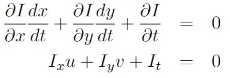
\includegraphics{eq1_r4.jpg}
\caption{caption}
\end{figure}

And the derivatives above can be expressed with \(h=1\) into:
\textbackslash{}begin\{aligned\} I\_x \&=
\frac{I(x+1, y) - I(x-1, y)}{2} \textbackslash{} I\_y \&=
\frac{I(x, y+1) - I(x, y-1)}{2} \textbackslash{}
\textbackslash{}end\{aligned\} \(I_t\) is simplified with only two
frames as: \[I_t = I(x, t+1) - I(x, t)\]

    This problem therefore becomes a least square problem, we have a
equation to solve the motion: 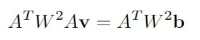
\includegraphics{eq2_r2.jpg} where
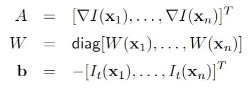
\includegraphics{eq3_r4.jpg}

    As a Ax=b problem, we can easily solve the motion matrix v using some
build-in functions in python.

However, this is only the gradient calculation in one grid while
computation in different grids are needed. Therefore, a function needs
to be developed to fill all the motion information into the matrices.
With these matrices, we are able to plot the optical flow.

    \hypertarget{implement}{%
\section{Implement}\label{implement}}

    The example below demonstrates the gradient method for displaying the
optical flow field by solving the least square problem with the motion
gradient constraint equation.

At the first beginning, several libraries which will be used is
imported.

    \begin{Verbatim}[commandchars=\\\{\}]
{\color{incolor}In [{\color{incolor}1}]:} \PY{k+kn}{import} \PY{n+nn}{numpy} \PY{k+kn}{as} \PY{n+nn}{np}
        \PY{k+kn}{import} \PY{n+nn}{matplotlib.pyplot} \PY{k+kn}{as} \PY{n+nn}{plt}
        \PY{k+kn}{from} \PY{n+nn}{skimage} \PY{k+kn}{import} \PY{n}{io}
\end{Verbatim}


    The image series are read in using io.imread. The first frame is called
I1 and the next frame is called I2. The motion is about to obtain by
comparing and calculating based on these two frames.

    \begin{Verbatim}[commandchars=\\\{\}]
{\color{incolor}In [{\color{incolor}2}]:} \PY{n}{seq1} \PY{o}{=} \PY{p}{\PYZob{}}\PY{l+s+s1}{\PYZsq{}}\PY{l+s+s1}{I1}\PY{l+s+s1}{\PYZsq{}}\PY{p}{:} \PY{n}{io}\PY{o}{.}\PY{n}{imread}\PY{p}{(}\PY{l+s+s1}{\PYZsq{}}\PY{l+s+s1}{data/image/seq1/frame1.png}\PY{l+s+s1}{\PYZsq{}}\PY{p}{,} \PY{n}{as\PYZus{}grey}\PY{o}{=}\PY{n+nb+bp}{True}\PY{p}{)}\PY{p}{,} 
                \PY{l+s+s1}{\PYZsq{}}\PY{l+s+s1}{I2}\PY{l+s+s1}{\PYZsq{}}\PY{p}{:} \PY{n}{io}\PY{o}{.}\PY{n}{imread}\PY{p}{(}\PY{l+s+s1}{\PYZsq{}}\PY{l+s+s1}{data/image/seq1/frame3.png}\PY{l+s+s1}{\PYZsq{}}\PY{p}{,} \PY{n}{as\PYZus{}grey}\PY{o}{=}\PY{n+nb+bp}{True}\PY{p}{)}\PY{p}{,}
                \PY{l+s+s1}{\PYZsq{}}\PY{l+s+s1}{U}\PY{l+s+s1}{\PYZsq{}} \PY{p}{:} \PY{n}{np}\PY{o}{.}\PY{n}{loadtxt}\PY{p}{(}\PY{l+s+s1}{\PYZsq{}}\PY{l+s+s1}{data/flow/seq1/flow3.u}\PY{l+s+s1}{\PYZsq{}}\PY{p}{,} \PY{n}{dtype}\PY{o}{=}\PY{l+s+s1}{\PYZsq{}}\PY{l+s+s1}{double}\PY{l+s+s1}{\PYZsq{}}\PY{p}{,} \PY{n}{delimiter}\PY{o}{=}\PY{l+s+s1}{\PYZsq{}}\PY{l+s+s1}{,}\PY{l+s+s1}{\PYZsq{}}\PY{p}{)}\PY{p}{,}
                \PY{l+s+s1}{\PYZsq{}}\PY{l+s+s1}{V}\PY{l+s+s1}{\PYZsq{}} \PY{p}{:} \PY{n}{np}\PY{o}{.}\PY{n}{loadtxt}\PY{p}{(}\PY{l+s+s1}{\PYZsq{}}\PY{l+s+s1}{data/flow/seq1/flow3.v}\PY{l+s+s1}{\PYZsq{}}\PY{p}{,} \PY{n}{dtype}\PY{o}{=}\PY{l+s+s1}{\PYZsq{}}\PY{l+s+s1}{double}\PY{l+s+s1}{\PYZsq{}}\PY{p}{,} \PY{n}{delimiter}\PY{o}{=}\PY{l+s+s1}{\PYZsq{}}\PY{l+s+s1}{,}\PY{l+s+s1}{\PYZsq{}}\PY{p}{)}\PY{p}{\PYZcb{}}
        
        \PY{n}{rubic} \PY{o}{=} \PY{p}{\PYZob{}}\PY{l+s+s1}{\PYZsq{}}\PY{l+s+s1}{I1}\PY{l+s+s1}{\PYZsq{}}\PY{p}{:}\PY{n}{io}\PY{o}{.}\PY{n}{imread}\PY{p}{(}\PY{l+s+s1}{\PYZsq{}}\PY{l+s+s1}{data/rubic/rubic.0.png}\PY{l+s+s1}{\PYZsq{}}\PY{p}{,} \PY{n}{as\PYZus{}grey}\PY{o}{=}\PY{n+nb+bp}{True}\PY{p}{)}\PY{p}{,} 
                 \PY{l+s+s1}{\PYZsq{}}\PY{l+s+s1}{I2}\PY{l+s+s1}{\PYZsq{}}\PY{p}{:}\PY{n}{io}\PY{o}{.}\PY{n}{imread}\PY{p}{(}\PY{l+s+s1}{\PYZsq{}}\PY{l+s+s1}{data/rubic/rubic.5.png}\PY{l+s+s1}{\PYZsq{}}\PY{p}{,} \PY{n}{as\PYZus{}grey}\PY{o}{=}\PY{n+nb+bp}{True}\PY{p}{)}\PY{p}{\PYZcb{}}
        
        \PY{n}{sphere}\PY{o}{=} \PY{p}{\PYZob{}}\PY{l+s+s1}{\PYZsq{}}\PY{l+s+s1}{I1}\PY{l+s+s1}{\PYZsq{}}\PY{p}{:} \PY{n}{io}\PY{o}{.}\PY{n}{imread}\PY{p}{(}\PY{l+s+s1}{\PYZsq{}}\PY{l+s+s1}{data/sphere/sphere.1.png}\PY{l+s+s1}{\PYZsq{}}\PY{p}{,} \PY{n}{as\PYZus{}grey}\PY{o}{=}\PY{n+nb+bp}{True}\PY{p}{)}\PY{p}{,} 
                 \PY{l+s+s1}{\PYZsq{}}\PY{l+s+s1}{I2}\PY{l+s+s1}{\PYZsq{}}\PY{p}{:} \PY{n}{io}\PY{o}{.}\PY{n}{imread}\PY{p}{(}\PY{l+s+s1}{\PYZsq{}}\PY{l+s+s1}{data/sphere/sphere.3.png}\PY{l+s+s1}{\PYZsq{}}\PY{p}{,} \PY{n}{as\PYZus{}grey}\PY{o}{=}\PY{n+nb+bp}{True}\PY{p}{)}\PY{p}{\PYZcb{}}
\end{Verbatim}


    \hypertarget{discrete-derivative-components-computation}{%
\subsection{Discrete Derivative Components
Computation}\label{discrete-derivative-components-computation}}

    The image is seperated into grids and a self-defined function is
developed to calculate the derivative components, \(I_x\),\(I_y\) and
\(I_t\), on each grid location based on \textbackslash{}begin\{aligned\}
I\_x \&= \frac{I(x+1, y) - I(x-1, y)}{2} \textbackslash{} I\_y \&=
\frac{I(x, y+1) - I(x, y-1)}{2} \textbackslash{}
\textbackslash{}end\{aligned\} \[I_t = I(x, t+1) - I(x, t)\]

Several boundary conditions should be satisfied to aviod the value going
beyond the reality.

    \begin{Verbatim}[commandchars=\\\{\}]
{\color{incolor}In [{\color{incolor}3}]:} \PY{k}{def} \PY{n+nf}{derivative\PYZus{}components}\PY{p}{(}\PY{n}{I1}\PY{p}{,} \PY{n}{I2}\PY{p}{,} \PY{n}{x\PYZus{}grid}\PY{p}{,} \PY{n}{y\PYZus{}grid}\PY{p}{)}\PY{p}{:}
            \PY{n}{h\PYZus{}img}\PY{o}{=} \PY{n}{I1}\PY{o}{.}\PY{n}{shape}\PY{p}{[}\PY{l+m+mi}{0}\PY{p}{]}
            \PY{n}{w\PYZus{}imd}\PY{o}{=} \PY{n}{I1}\PY{o}{.}\PY{n}{shape}\PY{p}{[}\PY{l+m+mi}{1}\PY{p}{]}
            \PY{n}{x\PYZus{}grid} \PY{o}{=} \PY{n+nb}{int}\PY{p}{(}\PY{n}{x\PYZus{}grid}\PY{p}{)}
            \PY{n}{y\PYZus{}grid} \PY{o}{=} \PY{n+nb}{int}\PY{p}{(}\PY{n}{y\PYZus{}grid}\PY{p}{)}
        
            \PY{k}{if} \PY{n}{x\PYZus{}grid}\PY{o}{\PYZgt{}}\PY{l+m+mi}{0} \PY{o+ow}{and} \PY{n}{x\PYZus{}grid}\PY{o}{\PYZlt{}} \PY{p}{(}\PY{n}{w\PYZus{}imd}\PY{o}{\PYZhy{}}\PY{l+m+mi}{1}\PY{p}{)} \PY{o+ow}{and} \PY{n}{y\PYZus{}grid}\PY{o}{\PYZgt{}}\PY{o}{=}\PY{l+m+mi}{0} \PY{o+ow}{and} \PY{n}{y\PYZus{}grid}\PY{o}{\PYZlt{}}\PY{n}{h\PYZus{}img}\PY{p}{:}
                \PY{n}{Ix}\PY{o}{=}\PY{p}{(}\PY{n}{I1}\PY{p}{[}\PY{n}{y\PYZus{}grid}\PY{p}{,} \PY{n}{x\PYZus{}grid}\PY{o}{+}\PY{l+m+mi}{1}\PY{p}{]} \PY{o}{\PYZhy{}} \PY{n}{I1}\PY{p}{[}\PY{n}{y\PYZus{}grid}\PY{p}{,} \PY{n}{x\PYZus{}grid}\PY{o}{\PYZhy{}}\PY{l+m+mi}{1}\PY{p}{]}\PY{p}{)}\PY{o}{/}\PY{l+m+mi}{2}\PY{p}{;}
            \PY{k}{else}\PY{p}{:}
                \PY{n}{Ix}\PY{o}{=}\PY{l+m+mi}{0}
        
            \PY{k}{if} \PY{n}{x\PYZus{}grid}\PY{o}{\PYZgt{}}\PY{o}{=}\PY{l+m+mi}{0} \PY{o+ow}{and} \PY{n}{x\PYZus{}grid}\PY{o}{\PYZlt{}}\PY{n}{w\PYZus{}imd} \PY{o+ow}{and} \PY{n}{y\PYZus{}grid}\PY{o}{\PYZgt{}}\PY{l+m+mi}{0} \PY{o+ow}{and} \PY{n}{y\PYZus{}grid}\PY{o}{\PYZlt{}} \PY{p}{(}\PY{n}{h\PYZus{}img}\PY{o}{\PYZhy{}}\PY{l+m+mi}{1}\PY{p}{)}\PY{p}{:}
                \PY{n}{Iy}\PY{o}{=}\PY{p}{(}\PY{n}{I1}\PY{p}{[}\PY{n}{y\PYZus{}grid}\PY{o}{+}\PY{l+m+mi}{1}\PY{p}{,} \PY{n}{x\PYZus{}grid}\PY{p}{]} \PY{o}{\PYZhy{}} \PY{n}{I1}\PY{p}{[}\PY{n}{y\PYZus{}grid}\PY{o}{\PYZhy{}}\PY{l+m+mi}{1}\PY{p}{,} \PY{n}{x\PYZus{}grid}\PY{p}{]}\PY{p}{)}\PY{o}{/}\PY{l+m+mi}{2}\PY{p}{;}
            \PY{k}{else}\PY{p}{:}
                \PY{n}{Iy}\PY{o}{=}\PY{l+m+mi}{0}
        
            \PY{k}{if} \PY{n}{x\PYZus{}grid}\PY{o}{\PYZgt{}}\PY{o}{=}\PY{l+m+mi}{0} \PY{o+ow}{and} \PY{n}{x\PYZus{}grid}\PY{o}{\PYZlt{}}\PY{n}{w\PYZus{}imd} \PY{o+ow}{and} \PY{n}{y\PYZus{}grid}\PY{o}{\PYZgt{}}\PY{o}{=}\PY{l+m+mi}{0} \PY{o+ow}{and} \PY{n}{y\PYZus{}grid}\PY{o}{\PYZlt{}}\PY{n}{h\PYZus{}img}\PY{p}{:}
                \PY{n}{It}\PY{o}{=}\PY{n}{I2}\PY{p}{[}\PY{n}{y\PYZus{}grid}\PY{p}{,}\PY{n}{x\PYZus{}grid}\PY{p}{]} \PY{o}{\PYZhy{}} \PY{n}{I1}\PY{p}{[}\PY{n}{y\PYZus{}grid}\PY{p}{,}\PY{n}{x\PYZus{}grid}\PY{p}{]}
            \PY{k}{else}\PY{p}{:}
                \PY{n}{It}\PY{o}{=}\PY{l+m+mi}{0}
        
            \PY{k}{return} \PY{p}{(}\PY{n}{Ix}\PY{p}{,} \PY{n}{Iy}\PY{p}{,} \PY{n}{It}\PY{p}{)}
\end{Verbatim}


    \hypertarget{matrix-a-and-vector-b-calculation-equation-solving-for-one-grid}{%
\subsection{Matrix A and Vector b Calculation \& Equation Solving for
one
grid}\label{matrix-a-and-vector-b-calculation-equation-solving-for-one-grid}}

    To calculate the motion matrix v, it should satisfy:
\[ A^T W^2 A v = A^T W^2 b \]

After simplifying, the equation looks like: \[ A v = b \]

where

\textbackslash{}begin\{aligned\} A \&= \textbackslash{}begin\{bmatrix\}
I\_x(x\_1) \& I\_y(x\_1) \textbackslash{} \dots \textbackslash{}
I\_x(x\_n) \& I\_y(x\_n) \textbackslash{}end\{bmatrix\} \textbackslash{}
b \&= -\textbackslash{}begin\{bmatrix\} I\_t(x\_1)\textbackslash{}
\dots\textbackslash{}
I\_t(x\_n)\textbackslash{}\textbackslash{}end\{bmatrix\}~
\textbackslash{}end\{aligned\}

And the v matrix can be obtained by np.linalg.lstsq() which returns the
least-squares solution to a linear matrix equation. The returned result
in this case is called motion\_estimation which is the v matrix.

    \begin{Verbatim}[commandchars=\\\{\}]
{\color{incolor}In [{\color{incolor}4}]:} \PY{k}{def} \PY{n+nf}{solve\PYZus{}motion\PYZus{}gradient\PYZus{}equation}\PY{p}{(}\PY{n}{I1}\PY{p}{,}\PY{n}{I2}\PY{p}{,}\PY{n}{x\PYZus{}grid}\PY{p}{,}\PY{n}{y\PYZus{}grid}\PY{p}{,}\PY{n}{width}\PY{p}{,}\PY{n}{disx}\PY{p}{,}\PY{n}{disy}\PY{p}{)}\PY{p}{:}
        
        
            \PY{n}{A} \PY{o}{=} \PY{n}{np}\PY{o}{.}\PY{n}{zeros}\PY{p}{(}\PY{p}{(}\PY{n}{width}\PY{o}{*}\PY{n}{width}\PY{p}{,} \PY{l+m+mi}{2}\PY{p}{)}\PY{p}{)}
            \PY{n}{b} \PY{o}{=} \PY{n}{np}\PY{o}{.}\PY{n}{zeros}\PY{p}{(}\PY{n}{width}\PY{o}{*}\PY{n}{width}\PY{p}{)}
            
        
        
            \PY{c+c1}{\PYZsh{} obtain A and b from I matrix}
            \PY{k}{for} \PY{n}{i} \PY{o+ow}{in} \PY{n+nb}{range}\PY{p}{(}\PY{l+m+mi}{0}\PY{p}{,} \PY{n}{width}\PY{o}{*}\PY{n}{width}\PY{p}{)}\PY{p}{:}
        
                \PY{n}{x\PYZus{}grid\PYZus{}m}\PY{o}{=} \PY{n}{x\PYZus{}grid}\PY{o}{+}\PY{n}{disx}\PY{p}{[}\PY{n}{i}\PY{p}{]}
                \PY{n}{y\PYZus{}grid\PYZus{}m}\PY{o}{=} \PY{n}{y\PYZus{}grid}\PY{o}{+}\PY{n}{disy}\PY{p}{[}\PY{n}{i}\PY{p}{]}
        
                \PY{n}{Ix}\PY{p}{,} \PY{n}{Iy}\PY{p}{,} \PY{n}{It} \PY{o}{=} \PY{n}{derivative\PYZus{}components}\PY{p}{(}\PY{n}{I1}\PY{p}{,} \PY{n}{I2}\PY{p}{,} \PY{n}{x\PYZus{}grid\PYZus{}m}\PY{p}{,} \PY{n}{y\PYZus{}grid\PYZus{}m}\PY{p}{)}
                \PY{n}{A}\PY{p}{[}\PY{n}{i}\PY{p}{,} \PY{l+m+mi}{0}\PY{p}{]} \PY{o}{=} \PY{n}{Ix} 
                \PY{n}{A}\PY{p}{[}\PY{n}{i}\PY{p}{,} \PY{l+m+mi}{1}\PY{p}{]} \PY{o}{=} \PY{n}{Iy}
                \PY{n}{b}\PY{p}{[}\PY{n}{i}\PY{p}{]} \PY{o}{=} \PY{o}{\PYZhy{}}\PY{n}{It}
        
            \PY{n}{motion\PYZus{}matrix} \PY{o}{=} \PY{n}{np}\PY{o}{.}\PY{n}{linalg}\PY{o}{.}\PY{n}{lstsq}\PY{p}{(}\PY{n}{np}\PY{o}{.}\PY{n}{matmul}\PY{p}{(}\PY{n}{A}\PY{o}{.}\PY{n}{T}\PY{p}{,} \PY{n}{A}\PY{p}{)}\PY{p}{,} \PY{n}{np}\PY{o}{.}\PY{n}{matmul}\PY{p}{(}\PY{n}{A}\PY{o}{.}\PY{n}{T}\PY{p}{,} \PY{n}{b}\PY{p}{)}\PY{p}{)}
        
            \PY{n}{motion\PYZus{}estimation} \PY{o}{=} \PY{n}{motion\PYZus{}matrix}\PY{p}{[}\PY{l+m+mi}{0}\PY{p}{]}
            
            \PY{k}{return} \PY{n}{motion\PYZus{}estimation}
\end{Verbatim}


    \hypertarget{motion-estimation-for-the-whole-image}{%
\subsection{Motion Estimation for the whole
image}\label{motion-estimation-for-the-whole-image}}

    The motion\_estimation obtained above is only for one grid. However, the
image consists of numerous of grids. One iteration is needed to fill all
the motion vector into matrices that express the motion in the whole
image.

    \begin{Verbatim}[commandchars=\\\{\}]
{\color{incolor}In [{\color{incolor}5}]:} \PY{k}{def} \PY{n+nf}{estimate\PYZus{}flow}\PY{p}{(}\PY{n}{img\PYZus{}series}\PY{p}{)}\PY{p}{:}
            \PY{c+c1}{\PYZsh{} get the image size.}
            \PY{n}{h\PYZus{}img} \PY{o}{=} \PY{n}{img\PYZus{}series}\PY{p}{[}\PY{l+s+s1}{\PYZsq{}}\PY{l+s+s1}{I1}\PY{l+s+s1}{\PYZsq{}}\PY{p}{]}\PY{o}{.}\PY{n}{shape}\PY{p}{[}\PY{l+m+mi}{0}\PY{p}{]}
            \PY{n}{w\PYZus{}img}\PY{o}{=} \PY{n}{img\PYZus{}series}\PY{p}{[}\PY{l+s+s1}{\PYZsq{}}\PY{l+s+s1}{I1}\PY{l+s+s1}{\PYZsq{}}\PY{p}{]}\PY{o}{.}\PY{n}{shape}\PY{p}{[}\PY{l+m+mi}{1}\PY{p}{]}
        
            \PY{c+c1}{\PYZsh{} define the grid size}
            \PY{n}{grid\PYZus{}size} \PY{o}{=} \PY{l+m+mi}{9}
            \PY{n}{width}  \PY{o}{=} \PY{l+m+mi}{21}
        
            \PY{c+c1}{\PYZsh{} x, y are the locations of the grids.}
            \PY{n}{x} \PY{o}{=} \PY{n}{np}\PY{o}{.}\PY{n}{arange}\PY{p}{(}\PY{l+m+mi}{0}\PY{p}{,} \PY{n}{w\PYZus{}img}\PY{o}{\PYZhy{}}\PY{n}{grid\PYZus{}size}\PY{p}{,} \PY{n}{grid\PYZus{}size}\PY{p}{)} \PY{o}{+} \PY{n}{np}\PY{o}{.}\PY{n}{floor}\PY{p}{(}\PY{n}{grid\PYZus{}size}\PY{o}{/}\PY{l+m+mi}{2}\PY{p}{)}\PY{p}{;}
            \PY{n}{y} \PY{o}{=} \PY{n}{np}\PY{o}{.}\PY{n}{arange}\PY{p}{(}\PY{l+m+mi}{0}\PY{p}{,} \PY{n}{h\PYZus{}img}\PY{o}{\PYZhy{}}\PY{n}{grid\PYZus{}size}\PY{p}{,} \PY{n}{grid\PYZus{}size}\PY{p}{)} \PY{o}{+} \PY{n}{np}\PY{o}{.}\PY{n}{floor}\PY{p}{(}\PY{n}{grid\PYZus{}size}\PY{o}{/}\PY{l+m+mi}{2}\PY{p}{)}\PY{p}{;}
        
         
            \PY{n}{x\PYZus{}grid}\PY{p}{,} \PY{n}{y\PYZus{}grid} \PY{o}{=} \PY{n}{np}\PY{o}{.}\PY{n}{meshgrid}\PY{p}{(}\PY{n}{x}\PY{p}{,}\PY{n}{y}\PY{p}{)}\PY{p}{;}
        
            
            \PY{c+c1}{\PYZsh{} get the height and width of the grid}
            \PY{n}{h\PYZus{}grid}\PY{o}{=} \PY{n}{x\PYZus{}grid}\PY{o}{.}\PY{n}{shape}\PY{p}{[}\PY{l+m+mi}{0}\PY{p}{]}
            \PY{n}{w\PYZus{}grid}\PY{o}{=} \PY{n}{x\PYZus{}grid}\PY{o}{.}\PY{n}{shape}\PY{p}{[}\PY{l+m+mi}{1}\PY{p}{]}  
           
            \PY{n}{U} \PY{o}{=} \PY{n}{np}\PY{o}{.}\PY{n}{zeros}\PY{p}{(}\PY{p}{(}\PY{n}{h\PYZus{}grid}\PY{p}{,} \PY{n}{w\PYZus{}grid}\PY{p}{)}\PY{p}{)}
            \PY{n}{V} \PY{o}{=} \PY{n}{np}\PY{o}{.}\PY{n}{zeros}\PY{p}{(}\PY{p}{(}\PY{n}{h\PYZus{}grid}\PY{p}{,} \PY{n}{w\PYZus{}grid}\PY{p}{)}\PY{p}{)}
        
            \PY{n}{grid\PYZus{}center} \PY{o}{=} \PY{n}{np}\PY{o}{.}\PY{n}{arange}\PY{p}{(}\PY{l+m+mi}{0}\PY{p}{,} \PY{n}{width}\PY{p}{)} \PY{o}{\PYZhy{}} \PY{n}{np}\PY{o}{.}\PY{n}{floor}\PY{p}{(}\PY{n}{width}\PY{o}{/}\PY{l+m+mi}{2}\PY{p}{)}
            \PY{n}{disx}\PY{p}{,} \PY{n}{disy} \PY{o}{=} \PY{n}{np}\PY{o}{.}\PY{n}{meshgrid}\PY{p}{(}\PY{n}{grid\PYZus{}center}\PY{p}{,} \PY{n}{grid\PYZus{}center}\PY{p}{)}
            \PY{n}{disx} \PY{o}{=} \PY{n}{disx}\PY{o}{.}\PY{n}{reshape}\PY{p}{(}\PY{n}{width}\PY{o}{*}\PY{n}{width}\PY{p}{,} \PY{l+m+mi}{1}\PY{p}{)}
            \PY{n}{disy} \PY{o}{=} \PY{n}{disy}\PY{o}{.}\PY{n}{reshape}\PY{p}{(}\PY{n}{width}\PY{o}{*}\PY{n}{width}\PY{p}{,} \PY{l+m+mi}{1}\PY{p}{)}
        
            
            \PY{c+c1}{\PYZsh{} get the U,V matrix}
            \PY{k}{for} \PY{n}{i} \PY{o+ow}{in} \PY{n+nb}{range}\PY{p}{(}\PY{l+m+mi}{0}\PY{p}{,} \PY{n}{h\PYZus{}grid}\PY{p}{)}\PY{p}{:}
                \PY{k}{for} \PY{n}{j} \PY{o+ow}{in} \PY{n+nb}{range}\PY{p}{(}\PY{l+m+mi}{0}\PY{p}{,} \PY{n}{w\PYZus{}grid}\PY{p}{)}\PY{p}{:}
                    \PY{c+c1}{\PYZsh{} x\PYZus{}grid[i,j] is the x coordinate; y\PYZus{}grid[i,j] is the y coordinate.}
                    \PY{n}{motion\PYZus{}estimation} \PY{o}{=}  \PY{n}{solve\PYZus{}motion\PYZus{}gradient\PYZus{}equation}\PY{p}{(}\PY{n}{img\PYZus{}series}\PY{p}{[}\PY{l+s+s2}{\PYZdq{}}\PY{l+s+s2}{I1}\PY{l+s+s2}{\PYZdq{}}\PY{p}{]}\PY{p}{,} \PY{n}{img\PYZus{}series}\PY{p}{[}\PY{l+s+s2}{\PYZdq{}}\PY{l+s+s2}{I2}\PY{l+s+s2}{\PYZdq{}}\PY{p}{]}\PY{p}{,}
                                                                        \PY{n}{x\PYZus{}grid}\PY{p}{[}\PY{n}{i}\PY{p}{,}\PY{n}{j}\PY{p}{]}\PY{p}{,} \PY{n}{y\PYZus{}grid}\PY{p}{[}\PY{n}{i}\PY{p}{,}\PY{n}{j}\PY{p}{]}\PY{p}{,} \PY{n}{width}\PY{p}{,}\PY{n}{disx}\PY{p}{,}\PY{n}{disy}\PY{p}{)}
                    \PY{n}{U}\PY{p}{[}\PY{n}{i}\PY{p}{,} \PY{n}{j}\PY{p}{]} \PY{o}{=} \PY{n}{motion\PYZus{}estimat} \PY{o}{\PYZam{}}\PY{n}{ion}\PY{p}{[}\PY{l+m+mi}{0}\PY{p}{]}
                    \PY{n}{V}\PY{p}{[}\PY{n}{i}\PY{p}{,} \PY{n}{j}\PY{p}{]} \PY{o}{=} \PY{n}{motion\PYZus{}estimation}\PY{p}{[}\PY{l+m+mi}{1}\PY{p}{]}
        
            \PY{n}{quiver\PYZus{}drawing}\PY{p}{(}\PY{n}{img\PYZus{}series}\PY{p}{[}\PY{l+s+s2}{\PYZdq{}}\PY{l+s+s2}{I1}\PY{l+s+s2}{\PYZdq{}}\PY{p}{]}\PY{p}{,} \PY{n}{x}\PY{p}{,} \PY{n}{y}\PY{p}{,} \PY{n}{U}\PY{p}{,} \PY{n}{V}\PY{p}{,} \PY{l+m+mi}{5}\PY{p}{)}
\end{Verbatim}


    \hypertarget{optical-flow-field-display}{%
\subsection{Optical Flow Field
Display}\label{optical-flow-field-display}}

    A function called quiver\_drawing() in the last line has not been
explained yet. As its name, the function is built for drawing quivers to
display the optical flow field. The basic idea behind this is simply
that drawing quivers based on the grid locations, motion matrices
returned back from estimate\_flow() as well as a scale scalar.

    \begin{Verbatim}[commandchars=\\\{\}]
{\color{incolor}In [{\color{incolor}6}]:} \PY{k}{def} \PY{n+nf}{quiver\PYZus{}drawing}\PY{p}{(}\PY{n}{I}\PY{p}{,} \PY{n}{x\PYZus{}grid}\PY{p}{,} \PY{n}{y\PYZus{}grid}\PY{p}{,} \PY{n}{U}\PY{p}{,} \PY{n}{V}\PY{p}{,} \PY{n}{scale}\PY{p}{)}\PY{p}{:}
            \PY{n}{fig}\PY{p}{,} \PY{n}{ax} \PY{o}{=} \PY{n}{plt}\PY{o}{.}\PY{n}{subplots}\PY{p}{(}\PY{n}{figsize}\PY{o}{=}\PY{p}{(}\PY{l+m+mi}{10}\PY{p}{,} \PY{l+m+mi}{10}\PY{p}{)}\PY{p}{,} \PY{n}{dpi}\PY{o}{=}\PY{l+m+mi}{80}\PY{p}{)}
            \PY{n}{ax}\PY{o}{.}\PY{n}{imshow}\PY{p}{(}\PY{n}{I}\PY{p}{,} \PY{n}{cmap}\PY{o}{=}\PY{l+s+s1}{\PYZsq{}}\PY{l+s+s1}{gray}\PY{l+s+s1}{\PYZsq{}}\PY{p}{)}
            \PY{n}{ax}\PY{o}{.}\PY{n}{quiver}\PY{p}{(}\PY{n}{x\PYZus{}grid}\PY{p}{,} \PY{n}{y\PYZus{}grid}\PY{p}{,} \PY{n}{U}\PY{o}{*}\PY{n}{scale}\PY{p}{,} \PY{n}{V}\PY{o}{*}\PY{n}{scale}\PY{p}{,} \PY{n}{color}\PY{o}{=}\PY{l+s+s1}{\PYZsq{}}\PY{l+s+s1}{red}\PY{l+s+s1}{\PYZsq{}}\PY{p}{,} \PY{n}{angles}\PY{o}{=}\PY{l+s+s1}{\PYZsq{}}\PY{l+s+s1}{xy}\PY{l+s+s1}{\PYZsq{}}\PY{p}{,} \PY{n}{scale\PYZus{}units}\PY{o}{=}\PY{l+s+s1}{\PYZsq{}}\PY{l+s+s1}{xy}\PY{l+s+s1}{\PYZsq{}}\PY{p}{,} \PY{n}{scale}\PY{o}{=}\PY{l+m+mi}{1}\PY{p}{)}
            \PY{n}{ax}\PY{o}{.}\PY{n}{set\PYZus{}aspect}\PY{p}{(}\PY{l+s+s1}{\PYZsq{}}\PY{l+s+s1}{equal}\PY{l+s+s1}{\PYZsq{}}\PY{p}{)}
            \PY{n}{plt}\PY{o}{.}\PY{n}{show}\PY{p}{(}\PY{p}{)}
\end{Verbatim}


    Apply image series into the function to check the results.

    \begin{Verbatim}[commandchars=\\\{\}]
{\color{incolor}In [{\color{incolor}7}]:} \PY{n}{estimate\PYZus{}flow}\PY{p}{(}\PY{n}{rubic}\PY{p}{)}
\end{Verbatim}


    \begin{center}
    \adjustimage{max size={0.9\linewidth}{0.9\paperheight}}{output_23_0.png}
    \end{center}
    { \hspace*{\fill} \\}
    
    \begin{Verbatim}[commandchars=\\\{\}]
{\color{incolor}In [{\color{incolor}8}]:} \PY{n}{estimate\PYZus{}flow}\PY{p}{(}\PY{n}{sphere}\PY{p}{)}
\end{Verbatim}


    \begin{center}
    \adjustimage{max size={0.9\linewidth}{0.9\paperheight}}{output_24_0.png}
    \end{center}
    { \hspace*{\fill} \\}
    
    \begin{Verbatim}[commandchars=\\\{\}]
{\color{incolor}In [{\color{incolor}9}]:} \PY{n}{estimate\PYZus{}flow}\PY{p}{(}\PY{n}{seq1}\PY{p}{)}
\end{Verbatim}


    \begin{center}
    \adjustimage{max size={0.9\linewidth}{0.9\paperheight}}{output_25_0.png}
    \end{center}
    { \hspace*{\fill} \\}
    
    \hypertarget{comparison-between-gradient-method-and-correlation-method}{%
\subsection{Comparison between Gradient Method and Correlation
Method}\label{comparison-between-gradient-method-and-correlation-method}}

    The results from the correlation method are:
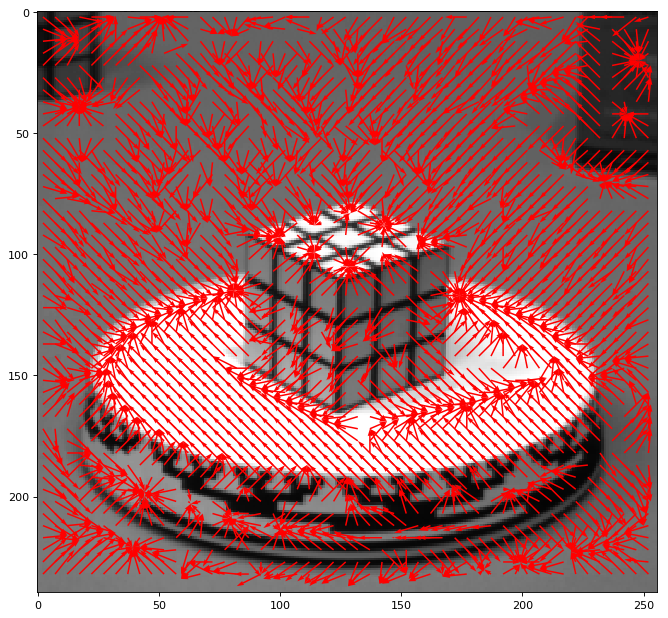
\includegraphics{output_16_0.png} 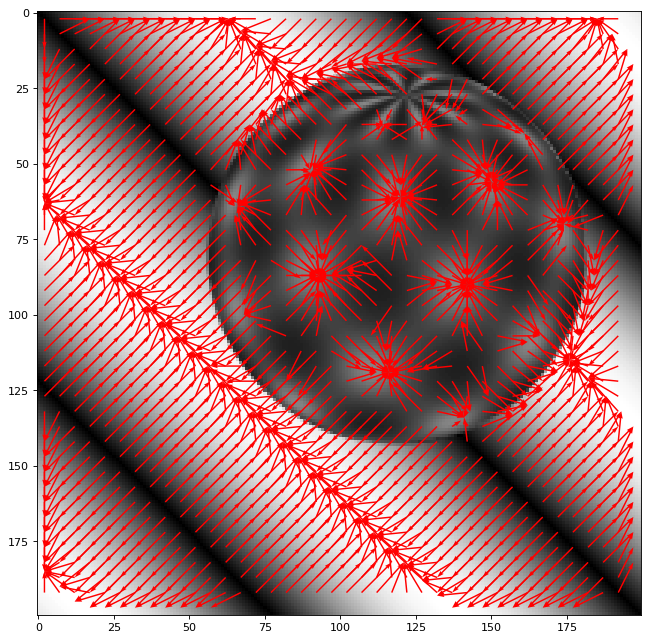
\includegraphics{output_15_0.png}
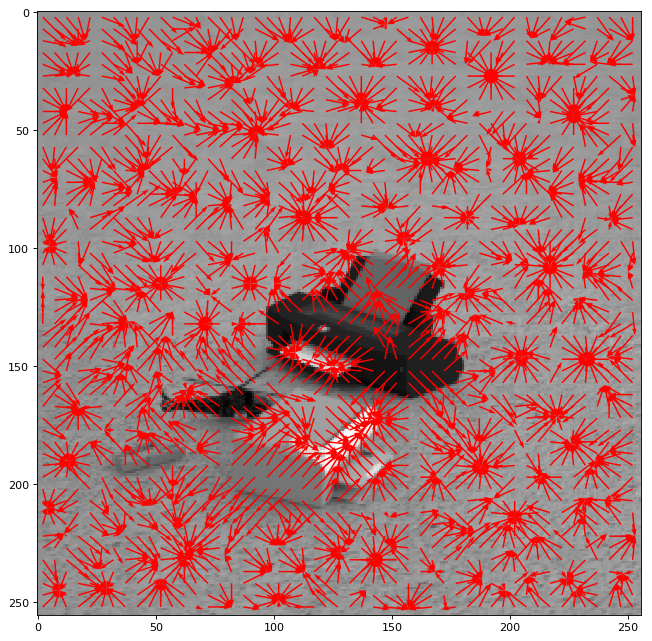
\includegraphics{output_17_0.png}

Compare these three optical flow field images with the results using
gradient and we can say that the gradient method definitely works
better. It is not saying that correlation method is worse than gradient
method in general. We have to admit that correlation method is
outstanding in some cases but not in these specific ones.

    \hypertarget{exploration}{%
\section{Exploration}\label{exploration}}

    From the results above, the estimated motion is meaning and does reflect
the correct direction of the movement. However, the background sometimes
is meaningless to be detected and wastes the computation storage while
people mostly focus on the objects. How about using the edge detector to
highlight the edge and then apply the gradient method to estimate the
motion? The code shown below is a demonstration for this idea.

    Take the rubic image series for an example. Use canny edge detector with
different threshold to do the image pre-processing.

    \begin{Verbatim}[commandchars=\\\{\}]
{\color{incolor}In [{\color{incolor}16}]:} \PY{k+kn}{import} \PY{n+nn}{cv2}
         
         \PY{n}{rubic\PYZus{}start}\PY{o}{=}\PY{n}{cv2}\PY{o}{.}\PY{n}{imread}\PY{p}{(}\PY{l+s+s1}{\PYZsq{}}\PY{l+s+s1}{data/rubic/rubic.0.png}\PY{l+s+s1}{\PYZsq{}}\PY{p}{)}
         \PY{n}{rubic\PYZus{}end}\PY{o}{=}\PY{n}{cv2}\PY{o}{.}\PY{n}{imread}\PY{p}{(}\PY{l+s+s1}{\PYZsq{}}\PY{l+s+s1}{data/rubic/rubic.5.png}\PY{l+s+s1}{\PYZsq{}}\PY{p}{)}
         
         \PY{c+c1}{\PYZsh{} canny edge detector, set different lower and upper thresholds for the detector.}
         \PY{n}{rubic\PYZus{}s300}\PY{o}{=}\PY{n}{cv2}\PY{o}{.}\PY{n}{Canny}\PY{p}{(}\PY{n}{rubic\PYZus{}start}\PY{p}{,}\PY{l+m+mi}{300}\PY{p}{,}\PY{l+m+mi}{300}\PY{p}{)}
         \PY{n}{rubic\PYZus{}e300}\PY{o}{=}\PY{n}{cv2}\PY{o}{.}\PY{n}{Canny}\PY{p}{(}\PY{n}{rubic\PYZus{}end}\PY{p}{,}\PY{l+m+mi}{300}\PY{p}{,}\PY{l+m+mi}{300}\PY{p}{)}
         \PY{n}{rubic\PYZus{}s400}\PY{o}{=}\PY{n}{cv2}\PY{o}{.}\PY{n}{Canny}\PY{p}{(}\PY{n}{rubic\PYZus{}start}\PY{p}{,}\PY{l+m+mi}{400}\PY{p}{,}\PY{l+m+mi}{400}\PY{p}{)}
         \PY{n}{rubic\PYZus{}e400}\PY{o}{=}\PY{n}{cv2}\PY{o}{.}\PY{n}{Canny}\PY{p}{(}\PY{n}{rubic\PYZus{}end}\PY{p}{,}\PY{l+m+mi}{400}\PY{p}{,}\PY{l+m+mi}{400}\PY{p}{)}
         \PY{n}{cv2}\PY{o}{.}\PY{n}{imwrite}\PY{p}{(}\PY{l+s+s1}{\PYZsq{}}\PY{l+s+s1}{rubic\PYZus{}s300.png}\PY{l+s+s1}{\PYZsq{}}\PY{p}{,}\PY{n}{rubic\PYZus{}s300}\PY{p}{)}
         \PY{n}{cv2}\PY{o}{.}\PY{n}{imwrite}\PY{p}{(}\PY{l+s+s1}{\PYZsq{}}\PY{l+s+s1}{rubic\PYZus{}e300.png}\PY{l+s+s1}{\PYZsq{}}\PY{p}{,}\PY{n}{rubic\PYZus{}e300}\PY{p}{)}
         \PY{n}{cv2}\PY{o}{.}\PY{n}{imwrite}\PY{p}{(}\PY{l+s+s1}{\PYZsq{}}\PY{l+s+s1}{rubic\PYZus{}s400.png}\PY{l+s+s1}{\PYZsq{}}\PY{p}{,}\PY{n}{rubic\PYZus{}s400}\PY{p}{)}
         \PY{n}{cv2}\PY{o}{.}\PY{n}{imwrite}\PY{p}{(}\PY{l+s+s1}{\PYZsq{}}\PY{l+s+s1}{rubic\PYZus{}e400.png}\PY{l+s+s1}{\PYZsq{}}\PY{p}{,}\PY{n}{rubic\PYZus{}e400}\PY{p}{)}
\end{Verbatim}


\begin{Verbatim}[commandchars=\\\{\}]
{\color{outcolor}Out[{\color{outcolor}16}]:} True
\end{Verbatim}
            
    Read the images in with io.image as the same as the previous step.

    \begin{Verbatim}[commandchars=\\\{\}]
{\color{incolor}In [{\color{incolor}17}]:} \PY{n}{rubic300} \PY{o}{=} \PY{p}{\PYZob{}}\PY{l+s+s1}{\PYZsq{}}\PY{l+s+s1}{I1}\PY{l+s+s1}{\PYZsq{}}\PY{p}{:}\PY{n}{io}\PY{o}{.}\PY{n}{imread}\PY{p}{(}\PY{l+s+s1}{\PYZsq{}}\PY{l+s+s1}{rubic\PYZus{}s300.png}\PY{l+s+s1}{\PYZsq{}}\PY{p}{,} \PY{n}{as\PYZus{}grey}\PY{o}{=}\PY{n+nb+bp}{True}\PY{p}{)}\PY{p}{,} 
                  \PY{l+s+s1}{\PYZsq{}}\PY{l+s+s1}{I2}\PY{l+s+s1}{\PYZsq{}}\PY{p}{:}\PY{n}{io}\PY{o}{.}\PY{n}{imread}\PY{p}{(}\PY{l+s+s1}{\PYZsq{}}\PY{l+s+s1}{rubic\PYZus{}e300.png}\PY{l+s+s1}{\PYZsq{}}\PY{p}{,} \PY{n}{as\PYZus{}grey}\PY{o}{=}\PY{n+nb+bp}{True}\PY{p}{)}\PY{p}{\PYZcb{}}
         \PY{n}{rubic400} \PY{o}{=} \PY{p}{\PYZob{}}\PY{l+s+s1}{\PYZsq{}}\PY{l+s+s1}{I1}\PY{l+s+s1}{\PYZsq{}}\PY{p}{:}\PY{n}{io}\PY{o}{.}\PY{n}{imread}\PY{p}{(}\PY{l+s+s1}{\PYZsq{}}\PY{l+s+s1}{rubic\PYZus{}s400.png}\PY{l+s+s1}{\PYZsq{}}\PY{p}{,} \PY{n}{as\PYZus{}grey}\PY{o}{=}\PY{n+nb+bp}{True}\PY{p}{)}\PY{p}{,} 
                  \PY{l+s+s1}{\PYZsq{}}\PY{l+s+s1}{I2}\PY{l+s+s1}{\PYZsq{}}\PY{p}{:}\PY{n}{io}\PY{o}{.}\PY{n}{imread}\PY{p}{(}\PY{l+s+s1}{\PYZsq{}}\PY{l+s+s1}{rubic\PYZus{}e400.png}\PY{l+s+s1}{\PYZsq{}}\PY{p}{,} \PY{n}{as\PYZus{}grey}\PY{o}{=}\PY{n+nb+bp}{True}\PY{p}{)}\PY{p}{\PYZcb{}}
\end{Verbatim}


    Test the image on the functions defined above.

    \begin{Verbatim}[commandchars=\\\{\}]
{\color{incolor}In [{\color{incolor}18}]:} \PY{n}{estimate\PYZus{}flow}\PY{p}{(}\PY{n}{rubic300}\PY{p}{)}
         \PY{n}{estimate\PYZus{}flow}\PY{p}{(}\PY{n}{rubic400}\PY{p}{)}
\end{Verbatim}


    \begin{Verbatim}[commandchars=\\\{\}]
/usr/local/lib/python2.7/dist-packages/ipykernel\_launcher.py:8: RuntimeWarning: overflow encountered in ubyte\_scalars
  
/usr/local/lib/python2.7/dist-packages/ipykernel\_launcher.py:13: RuntimeWarning: overflow encountered in ubyte\_scalars
  del sys.path[0]
/usr/local/lib/python2.7/dist-packages/ipykernel\_launcher.py:18: RuntimeWarning: overflow encountered in ubyte\_scalars

    \end{Verbatim}

    \begin{center}
    \adjustimage{max size={0.9\linewidth}{0.9\paperheight}}{output_35_1.png}
    \end{center}
    { \hspace*{\fill} \\}
    
    \begin{center}
    \adjustimage{max size={0.9\linewidth}{0.9\paperheight}}{output_35_2.png}
    \end{center}
    { \hspace*{\fill} \\}
    
    \hypertarget{conclusion-and-discussion}{%
\section{Conclusion and Discussion}\label{conclusion-and-discussion}}

    Motion is successfully estimated with gradient method which is basically
to solve the motion matrix using the motion gradient constraint equation
and least-square equation.The quivers correctly reflect the direction of
the object movement in three different image series. Compared with the
results obtained from correlation method, this optical flow field make
more sense and is more realistic.

As for the exploration, although the results are not as good as the ones
without applying edge detector, it illuminates how robust the gradient
method is. The values of the pixels in original images are from 0 to 255
while they are only 0 or 255 after pre-processing. In other words, most
of the information are lost during the processing. Surprisely, most of
the flow are still pointing to the correct direction. Moreover, without
annoying by the background, the movement of the object is shown
explicitly. Also, the results are slightly different with the changing
of the threshold of the canny edge detector.


    % Add a bibliography block to the postdoc
    
    
    
    \end{document}
